\documentclass{beamer}
\beamertemplatenavigationsymbolsempty
\usecolortheme{beaver}
\setbeamertemplate{blocks}[rounded=true, shadow=true]
\setbeamertemplate{footline}[page number]
%
\usepackage[utf8]{inputenc}
\usepackage[english]{babel}
\usepackage{amssymb,amsfonts,amsmath,mathtext}
\usepackage[]{algorithmic}
\usepackage{subfig}
\usepackage[all]{xy} % xy package for diagrams
\usepackage{array}
\usepackage{tikz}
\usepackage{multicol}% many columns in slide
\usepackage{hyperref}% urls
\usepackage{hhline}%tables
\usepackage{diagbox}

\newtheorem{hyp}{Hypothesis}


% Your figures are here:
\graphicspath{ {fig/} {../fig/} }

%----------------------------------------------------------------------------------------------------------
\title{Quantifying image realism via language model reasoning}
\author[K. Petrushina]{Kseniia~Petrushina}
\institute{Moscow Institute of Physics and Technology,\\ Skolkovo Institute of Science and Technology}

\date{\footnotesize

\par\smallskip\emph{Scientific supervisor:} Dr. Alexander~Panchenko
\par\bigskip\small 2024}
%----------------------------------------------------------------------------------------------------------
\begin{document}
%----------------------------------------------------------------------------------------------------------
\begin{frame}
\thispagestyle{empty}
\maketitle
\end{frame}
%-----------------------------------------------------------------------------------------------------
\begin{frame}{Purpose of the study}

\textbf{Problem}

As AI-generated images become more convincing, distinguishing realism from fiction is increasingly challenging.

\textbf{Goal}

Develop interpretable quantifiable realism measure to detect contextual and commonsense inconsistencies in visual content. 

\textbf{Tasks}
\begin{enumerate}
    \item Explore existing approaches in detecting image manipulation and realism.
    \item Develop a method for obtaining reality score using language model reasoning.
    \item Validate the method on a dataset of pairs of real and \textit{weird} images.
    \item Analyze the explanation of the \textit{weirdness} of the images.
\end{enumerate}

\end{frame}
%-----------------------------------------------------------------------------------------------------

\begin{frame}{Problem statement}

Given unknown \textit{real} and \textit{weird} probability distributions \[\mathrm{P}_\text{real}(\textbf{x}): \mathbb{R}^{n\times n} \to [0, 1] \quad \mathrm{P}_\text{weird}(\textbf{x}): \mathbb{R}^{n\times n} \to [0, 1]\]
and samples from the distributions
\[\mathcal{D}_\text{r} = \{\textbf{x}^i_\text{r}\;|\; \textbf{x}^i_\text{r} \sim \mathrm{P}_\text{real}(\textbf{x})\}_{i=1}^N\]
\[\mathcal{D}_\text{w} = \{\textbf{x}^i_\text{w}\;|\; \textbf{x}^i_\text{w}\sim \mathrm{P}_\text{weird}(\textbf{x})\}_{i=1}^N\]

\end{frame}
%----------------------------------------------------------------------------------------------------------

\begin{frame}{Problem statement}

We need to find a \textit{reality-check} function
\[\text{f}_\text{weird}: \mathbb{R}^{n\times n} \to \mathbb{R}_+\]
that defines the realism score, that is for \textit{real} image $\textbf{x}_\text{r}$ and \textit{weird} image $\textbf{x}_\text{w}$, provided that they are close in a sense of similarity measure $\langle \cdot, \cdot \rangle$:
\[ \langle \textbf{x}_\text{r}, \textbf{x}_\text{w}\rangle \le \varepsilon,\]
the following holds true
\[\text{f}_\text{weird}(\textbf{x}_\text{r}) < \text{f}_\text{weird}(\textbf{x}_\text{w}).\]


\end{frame}
%----------------------------------------------------------------------------------------------------------

\begin{frame}{Existing methods}

\begin{enumerate}
    \item \textbf{Probability}
    
    Realistic objects have high probability under distribution $\mathrm{P}$.

    \item \textbf{Weak typicality} \[\textbf{x}^N = (\textbf{x}_1, \dots, \textbf{x}_N) \overset{\mathrm{iid}}{\sim} \mathrm{P}\]
    \[\mathbb{P} \bigl[\lim\limits_{N \to \infty} -\dfrac1N \log \mathrm{P}(\textbf{x}^N) = H[\textbf{x}_n]\bigr] = 1\]
    \textit{Typical set} is \[A_\delta^N = \{\textbf{x}: | -\dfrac1N \log \mathrm{P}(\textbf{x}^N) - H[\textbf{x}_n]| < \delta \},\]
    its elements are \textit{weakly typical}.

\end{enumerate}

\end{frame}
%----------------------------------------------------------------------------------------------------------

\begin{frame}{Existing methods}

\begin{enumerate}
    \item[3.] \textbf{Adversarial losses} $f$-divergence between densities $p, q$
    \[D_f [q || p] \ge \mathbb{E}_q [T(\textbf{x})] - \mathbb{E}_p [f^* (T(\textbf{x}))]\]
    Real-valued function $T$ acts as a \textit{critic} and produces larger values for samples from $q$ and smaller for samples from $p$
    \item[4.] \textbf{Maximum mean discrepancy
} Given two sets of $\mathrm{iid}$ examples $\textbf{x}^M$, $\mathbf{\hat{x}}^N$ \[MMD^2 (\textbf{x}^M, \mathbf{\hat{x}}^N) = \| \frac1M \sum\limits_m \Phi(x_m) - \frac1N \sum\limits_n \Phi(\hat{x}_n) \|^2 \]
$\Phi$ is high dimensional feature space.
    \item[5.] \textbf{Universal critics}
    Measure of randomness to decide whether $\textbf{x}$ was drawn from $\mathrm{P}$: \[U(\textbf{x}) = -\log \mathrm{P}(\textbf{x}) - K(\textbf{x})\]
    $K(\textbf{x})$ is \textit{Kolmogorov complexity} of $\textbf{x}$.

\end{enumerate}

% The existing methods do not investigate whether there is enough information in $\mathbf{h}$ to restore $\mathbf{s}$.

\end{frame}
%----------------------------------------------------------------------------------------------------------

\begin{frame}{Proposed method}

% \textit{reality-check} function $\text{f}$ :

\textbf{Extracting atomic facts}

Using multi-modal model $\text{f}_\text{cap}: \mathbb{R}^{n\times n} \to \mathrm{T}^{m\times L}$ we obtain $m$ sequences of language tokens of length $L$, which describe the details about the image:
\[\text{f}_\text{cap}(\textbf{x}) = \mathrm{F}_\text{A} = \{[t^i_1, \dots, t^i_L]\;|\; i \in \overline{1, m} \} \]

\textbf{Pairwise natural language inference}

For each ordered pair of facts $(f_i, f_j) \in \mathrm{F}_\text{A} \times \mathrm{F}_\text{A}$ we calculate entailment score via $\text{f}_\text{nli}: \mathrm{T}^{L}\times \mathrm{T}^{L} \to [-1, 1]$.
The results are presented in the form of a matrix
\[S_{ij} = \text{f}_\text{nli}(f_i, f_j). \]

\textbf{Aggregating pairwise scores}

We take the sum of matrix elements, if both pairs $(f_i, f_j)$ and $(f_j, f_i)$ are contradictory and average it by the number of pairs:
\[\text{f}_\text{agg} (S) = - \dfrac{1}{m^2} \sum\limits_{i < j} (S_{ij} + S_{ji}) \mathbb{I} [S_{ij}, S_{ji} < 0] \]

\end{frame}
%----------------------------------------------------------------------------------------------------------

\begin{frame}{Proposed method}

\textbf{Resulting metric}

The final formula for \textit{reality-check} function is \[\text{f}_\text{weird} = \text{f}_\text{agg} \circ \text{f}_\text{nli} \circ \text{f}_\text{cap}\]

\begin{hyp}
Resulting reality scores $R = \{\text{f}_\text{weird}(\textbf{x})\}$ will correlate with probability densities $P = \{\mathrm{P}_\text{real} (\textbf{x})\}$:
\[\displaystyle r_{s} = \rho _{\operatorname {R} (\text{f}_\text{weird}(\textbf{x})),\operatorname {R} (\mathrm{P}_\text{real} (\textbf{x}))} \le -0.5\]
\end{hyp}
\end{frame}

\begin{frame}{Computational experiments}

\textbf{Data}

\begin{figure}
    \centering
  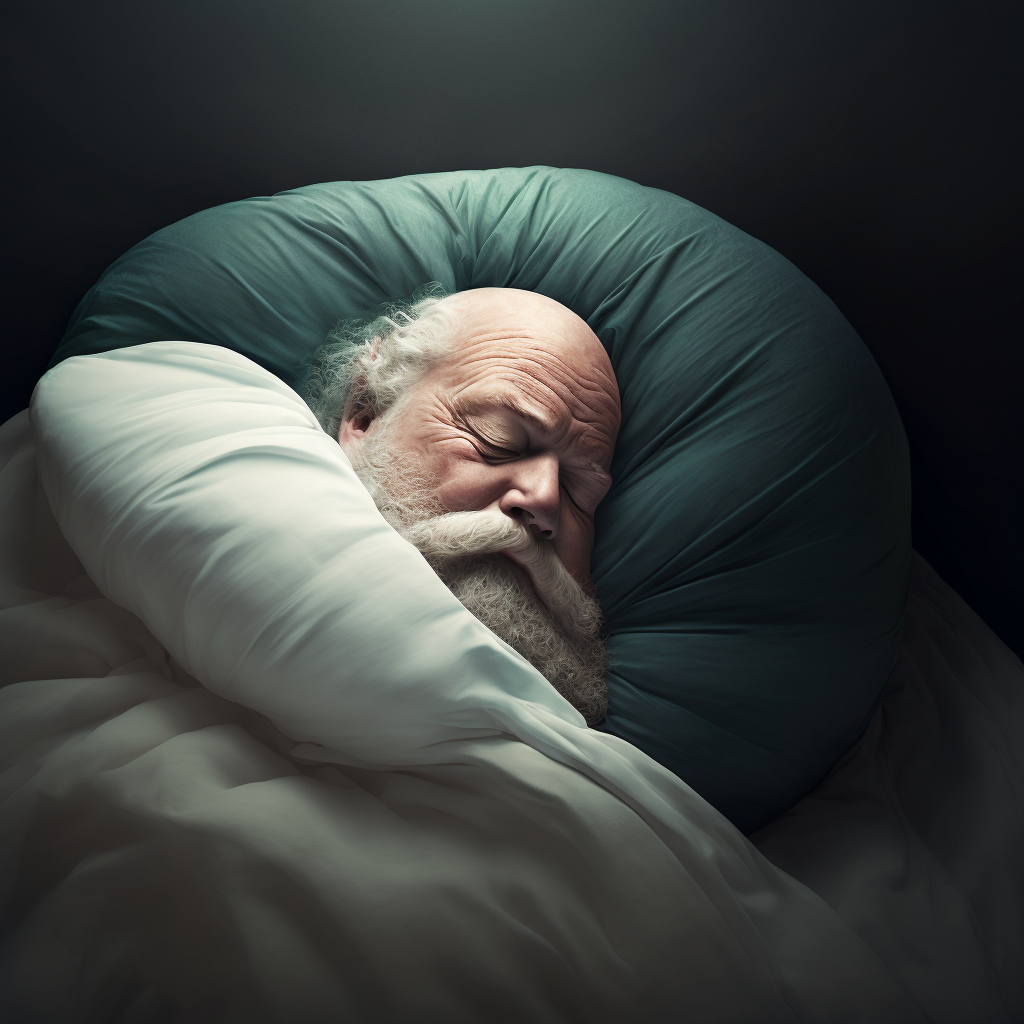
\includegraphics[width=0.3\linewidth]{images/sleep_1.png} 
  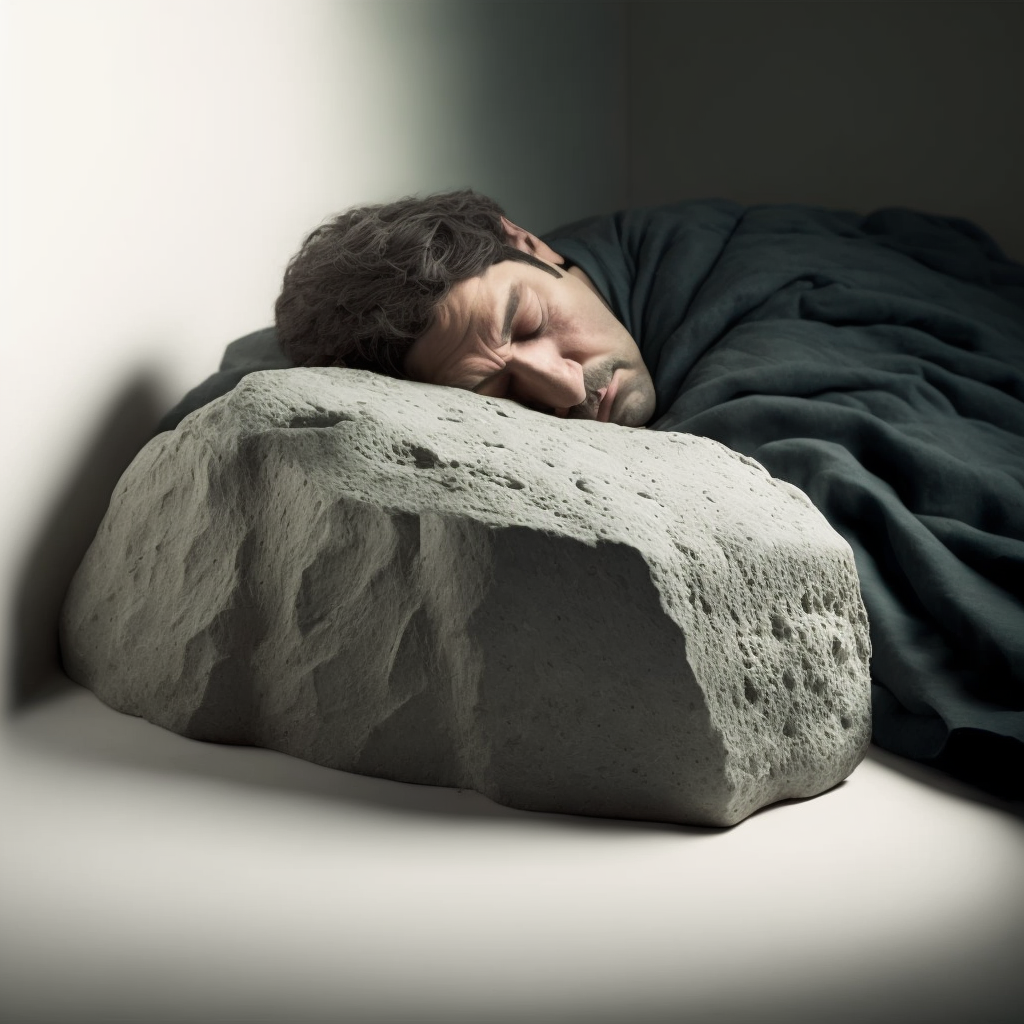
\includegraphics[width=0.3\linewidth]{images/sleep_0.png}
  \caption {Examples of \textit{real} and \textit{weird} images.}
  \label{fig:data}
\end{figure}

\textbf{Metrics}

\begin{enumerate}
    \item \[\text{Accuracy} = \frac1N \sum\limits_{i=1}^N \mathbb{I}[\text{f}_\text{weird}(\textbf{x}^i_r) < \text{f}_\text{weird}(\textbf{x}^i_w)]\]
    \item Spearman's rank correlation coefficient
    % \[r_s= \rho_{R(Y), R(\hat{Y})} = \frac{\text{cov} (R(Y), R(\hat{Y}))}{\sigma_{R(Y)} \sigma_{R(\hat{Y})}}\]
\end{enumerate}


\end{frame}
%----------------------------------------------------------------------------------------------------------

\begin{frame}{Results}

$\text{f}_\text{weird} = 0.31$

\begin{figure}[ht]
  \includegraphics[width=1.05\textwidth]{images/interpret_sleep_1.png}
  % \caption{}
  \label{fig:experiments}
\end{figure}
\end{frame}

\begin{frame}{Results}

$\text{f}_\text{weird} = 6.56$

\begin{figure}[ht]
  \includegraphics[width=1.05\textwidth]{images/interpret_sleep_0.png}
  % \caption{}
  \label{fig:experiments}
\end{figure}
\end{frame}

\begin{frame}{Results}

\begin{table}[ht]
    \centering
    \begin{tabular}{|c|c c c |}
        \hline
         \diagbox{$\text{f}_\text{cap}$}{$\text{f}_\text{nli}$} & sileod & MoritzLaurer & t5-true \\
         \hline
         LLaVa & \textbf{0.68} & 0.42 & 0.63 \\
         BLIP & 0.53 &\textbf{ 0.68} & 0.53 \\
         GPT-2 & 0.37 & 0.32 & 0.37 \\
         GPT-4o & 0.63 & \textbf{0.68} & 0.37 \\
         \hline
    \end{tabular}
    \caption{Accuracy of realistic images detection using various functions for $\text{f}_\text{cap}$ and $\text{f}_\text{nli}$.}
    \label{tab:acc}
\end{table}

\end{frame}

\begin{frame}{Results}

\begin{figure}[ht]
  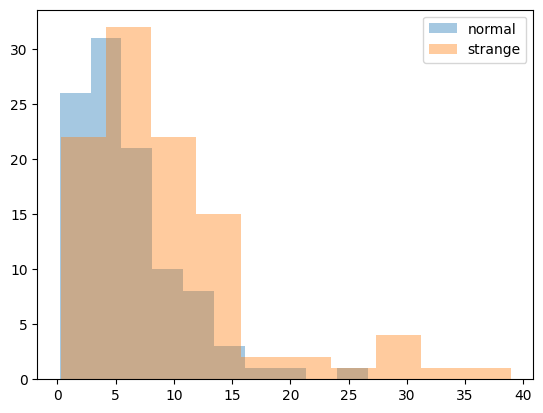
\includegraphics[width=0.8\textwidth]{images/output.png}
  \caption{Reality scores for the whole dataset obtained using \textit{LLaVa} model for captioning and \textit{sileod} model for contradiction detection. $p-value=4e-5$ for Kolmogorov–Smirnov test.}
  \label{fig:experiments}
\end{figure}

\end{frame}
%----------------------------------------------------------------------------------------------------------

%----------------------------------------------------------------------------------------------------------
\begin{frame}{Conclusion}
  \begin{itemize}
    \item Explored existing approaches in detecting image realism.
      \item Developed new interpretable method of quantifying image realism.
      \item Computational experiments on detecting \textit{weird} images with different configurations.
      \item Hypotheses about properties of the \textit{reality-check} function.
      
  \end{itemize}

  \textbf{Future work}: 
  \begin{itemize}
      \item Conduct experiments with measuring correlation with other methods.
      \item Analyse the interpretability of the proposed method in more details.
      \item Carry on comprehensive study of ablation.
  \end{itemize}
\end{frame}
%----------------------------------------------------------------------------------------------------------

\begin{frame}{Literature}
\begin{enumerate}
    \item Lucas Theis. 2024. \textcolor{blue}{What makes an image realistic?}. Proceedings of the 41st International Conference on Machine Learning.

    URL: \url{https://arxiv.org/abs/2403.04493}

    \item Sewon Min et al. 2023. \textcolor{blue}{{FA}ct{S}core: Fine-grained Atomic Evaluation of Factual Precision in Long Form Text Generation}. Association for Computational Linguistics.

    URL: \url{https://aclanthology.org/2023.emnlp-main.741}

    \item Nitzan Bitton-Guetta et al. 2023. \textcolor{blue}{Breaking Common Sense: WHOOPS! A Vision-and-Language Benchmark of Synthetic and Compositional Images}

    URL: \url{https://arxiv.org/abs/2303.07274}

  \end{enumerate}
\end{frame}
\end{document} 
